\documentclass{resume}
\usepackage{NotoSerifCJKsc_external}
\usepackage{linespacing_fix}
\usepackage{hyperref}
\usepackage{fontawesome}
\usepackage{graphicx}
\usepackage{booktabs} 

\begin{document}
\pagenumbering{gobble}

% --- 3+3 对称布局 ---
\noindent
\begin{minipage}[c][][c]{0.75\textwidth} % 左侧文字信息区
    
    \vspace*{0.5cm}

    % 使用 tabular 环境创建 3x2 对称网格
    \begin{tabular}{l@{\hspace{2.2cm}}l} % 列间距
        % 第一行
        \faUser\ 姓名:王健 & \faMapMarker\ 籍贯:江西 宜春 \\
        \addlinespace[3.5mm] % 行间距
        % 第二行
        \faEnvelope\ \href{mailto:jona.wzu@gmail.com}{jona.wzu@gmail.com} & \faBirthdayCake\ 出生年月:1999.04 \\
        \addlinespace[3.5mm]
        % 第三行
        \faPhone\ (+86) 157-7054-6370 & \faGithub\ \href{https://github.com/aajonaa}{https://github.com/aajonaa} \\ 
    \end{tabular}
    
    \vspace*{0.5cm}

\end{minipage}
\hspace{0.05\textwidth} % 与右侧照片的间距
\begin{minipage}[c][][c]{0.2\textwidth} % 右侧照片区
    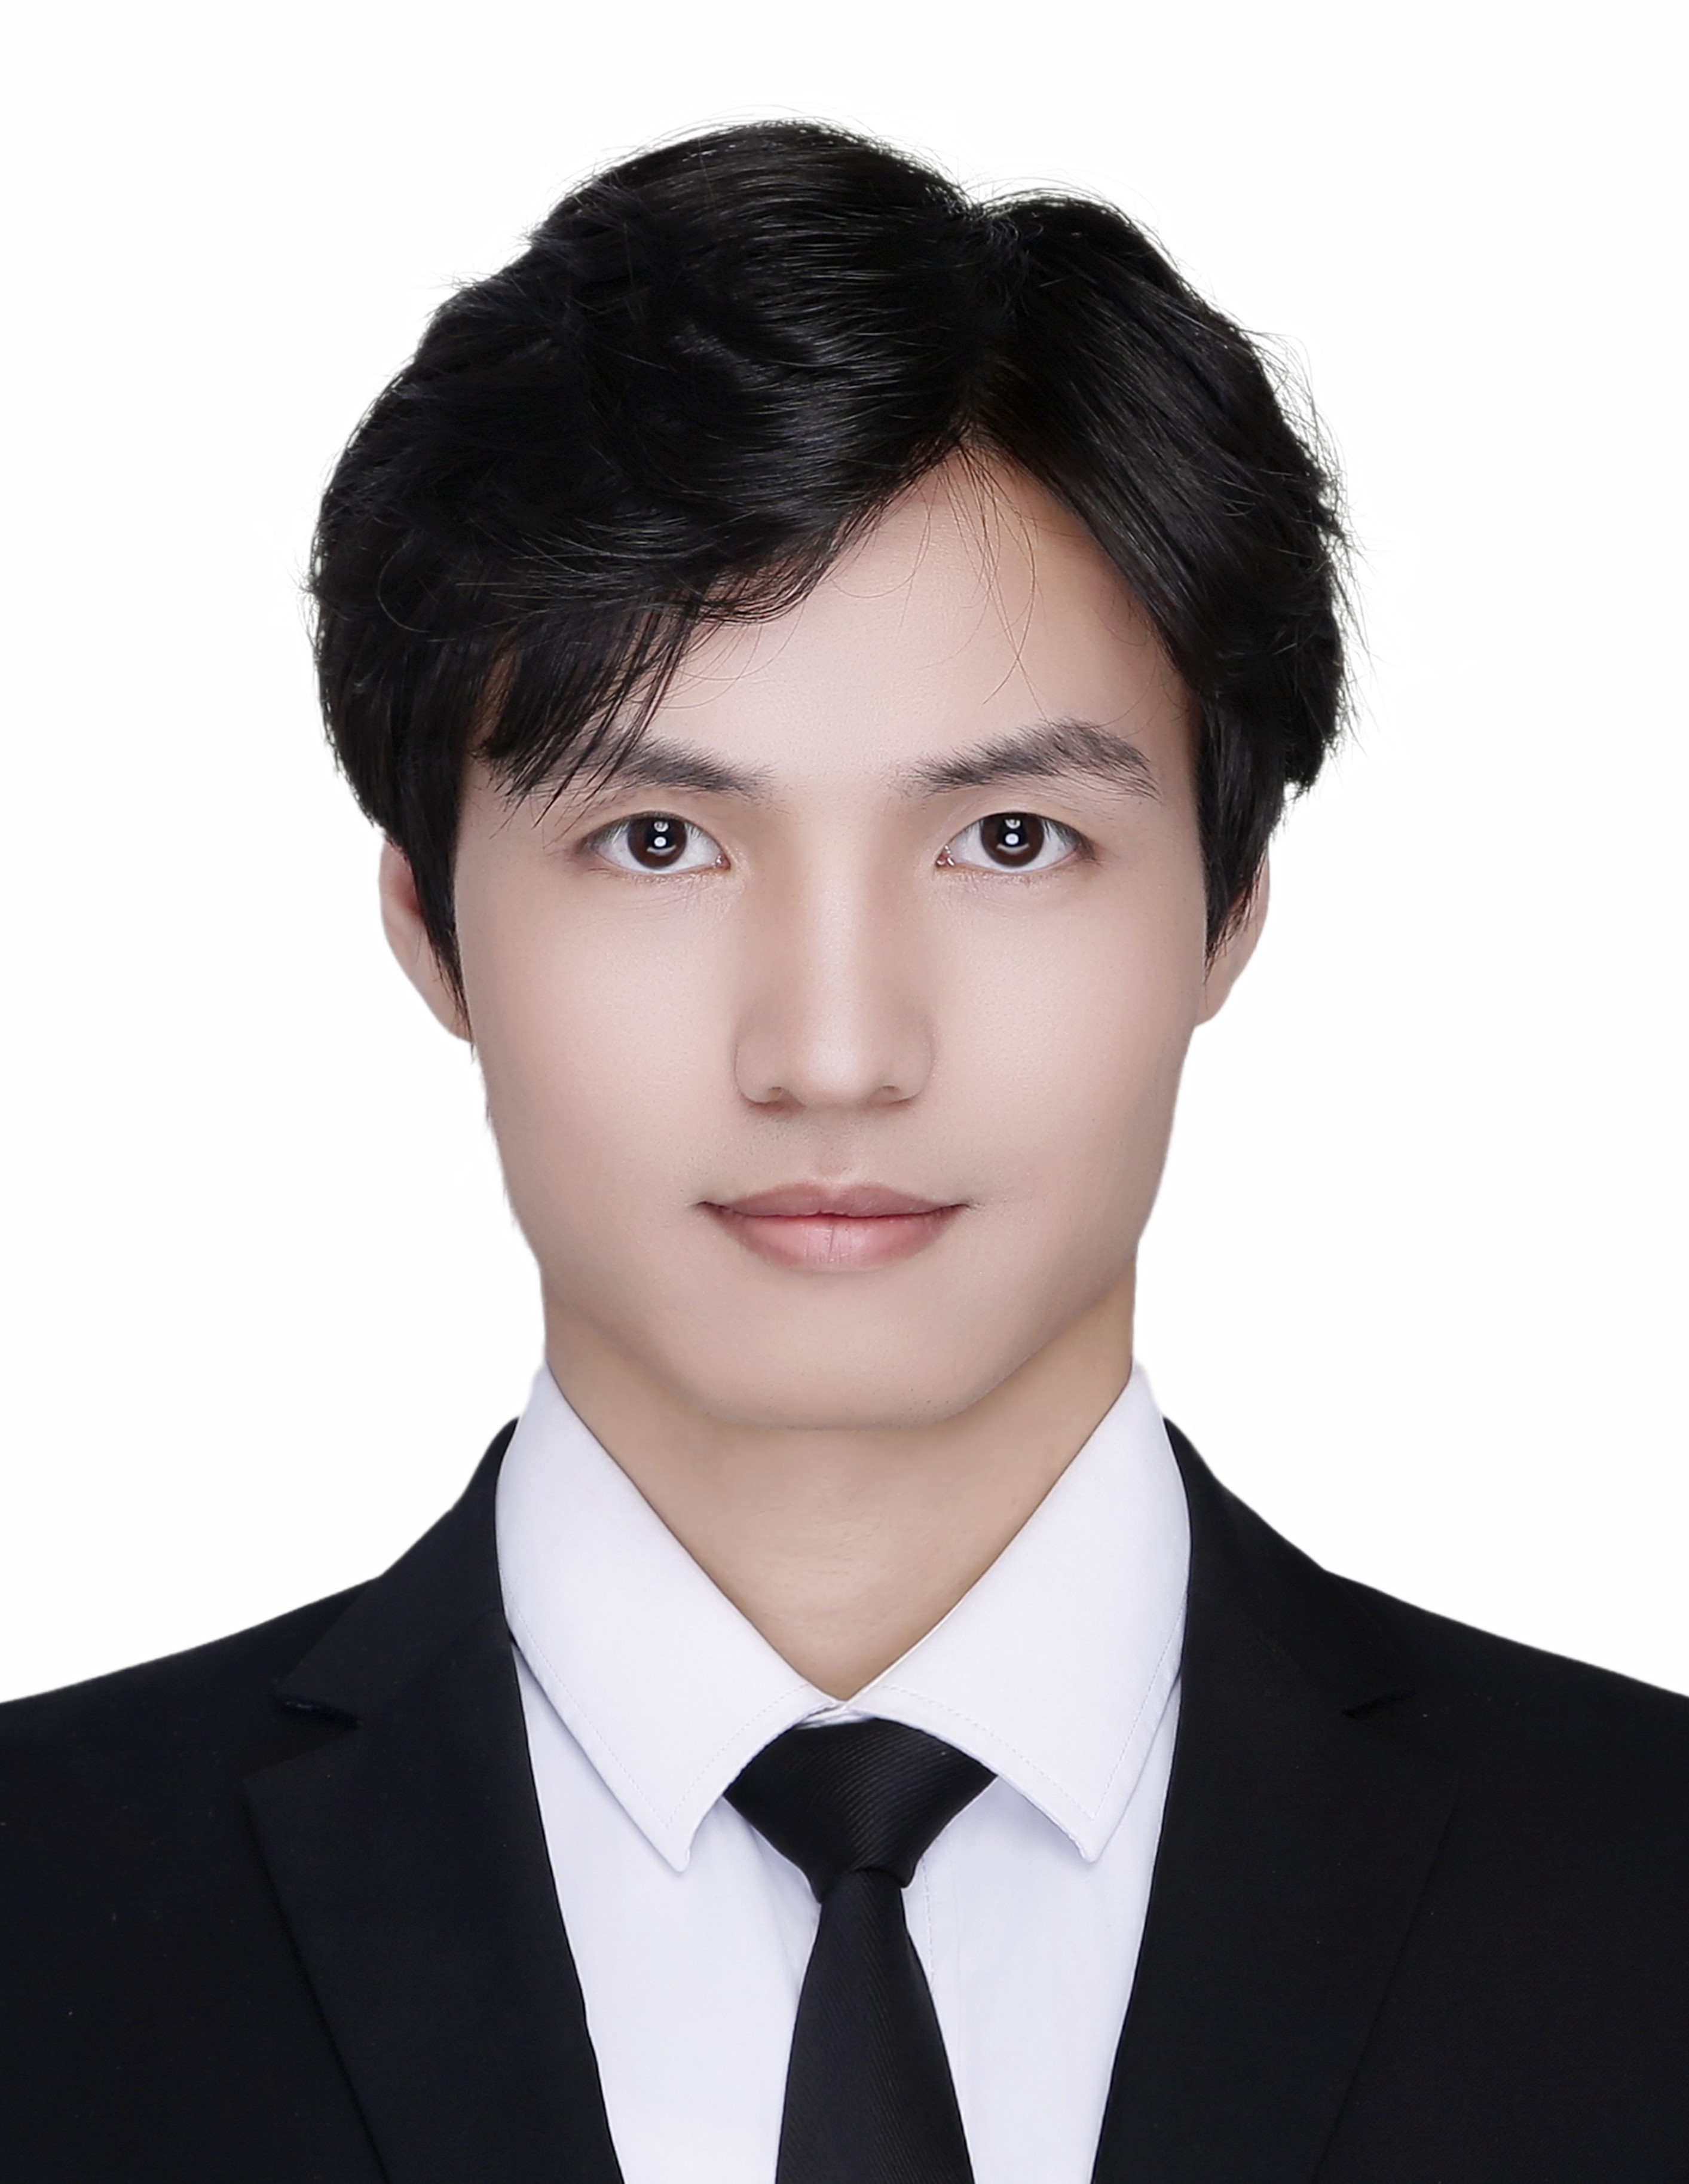
\includegraphics[width=\linewidth]{profile_2_mod.jpg} 
\end{minipage}

% --- 修改点:减小头部和正文之间的垂直距离 ---
\vspace{0.4cm} 
% --- 头部布局结束 ---

\section{\faInfoCircle\ 个人摘要}
硕士研究生,研究方向为演化计算与智能优化算法,已在该领域发表SCI二区论文。目前研究兴趣拓展至深度学习,关注自然语言处理(NLP)与计算机视觉(CV)中的通用建模方法,致力于探索演化优化方法与深度神经网络在泛化能力、跨模态建模与稳健学习中的融合路径。期望在博士阶段继续深入方法层面的研究与创新。

\section{\faGraduationCap\ 教育背景}
\datedsubsection{\textbf{温州大学}, 温州}{2023 -- 至今}
\textit{硕士研究生在读} \quad 计算机科学与技术 \quad 预计2026年6月毕业\\
导师:陈慧灵教授 课题组:医学数据挖掘与计算智能实验室

\datedsubsection{\textbf{江西理工大学}, 南昌}{2018 -- 2022}
\textit{工学学士} \quad 软件工程

\section{\faFileTextO\ 学术成果}
\begin{itemize}
  \item \textbf{Wang J}, Chen Y, Lu C, Heidari A A, Wu Z, Chen H.\\
  \textbf{The Status-based Optimization: Algorithm and Comprehensive Performance Analysis}.\\
  \textit{Neurocomputing}, 2025. (SCI二区, CCF-C, IF=6.5, JCR Q1)\\
  主导设计并实现\textbf{状态驱动优化(SBO)算法},创新性模拟社会个体地位竞争与资源分配机制,构建动态精英引导策略,显著提升多模态优化的收敛速度与种群多样性平衡能力。
  \item \textbf{Wang J}, Chen Y, Lu C, Heidari A A, Liu L, Chen H.\\
  \textbf{Bandit-Driven Adaptive Search in Surrogate-Assisted Evolutionary Algorithm with Explainable Uncertainty Criteria}.\\
  \textit{Swarm and Evolutionary Computation}, 2025. (SCI二区, IF=8.5, JCR Q1, 一审修改中)\\
  构建\textbf{BEXEA框架},首创性集成多臂老虎机动态平衡策略与可解释不确定性准则,实现代理辅助进化算法(SAEA)中搜索开发过程的自适应调控与模型决策透明化,显著降低高维黑盒优化问题的计算成本。
\end{itemize}

\section{\faKey\ 知识产权}
\begin{itemize}
  \item \textbf{发明专利}(第2发明人):一种多阈值图像分割方法、装置、计算机设备及存储介质\\
  申请号:2025110129939(受理中)
  \item \textbf{软件著作权}(3/5):基于深度学习模型的肺炎辅助诊断系统 V1.0\\
  登记号:2024SR1062875
\end{itemize}

\section{\faTrophy\ 获奖情况}
\begin{itemize}[parsep=0.5ex]
  \item \textbf{国家级:} 铜奖 (团队排名3/15), 第十四届“挑战杯”中国大学生创业计划竞赛“一带一路”国际邀请赛 | 2024
  \item \textbf{省级:} 银奖 (团队负责人), “建行杯”浙江省国际大学生创新大赛 | 2024
  \item \textbf{校级:} 金奖 (团队排名4/15), 温州大学第十一届“挑战杯”竞赛 | 2025
  \item \textbf{校级:} 温州大学一等奖学金 (排名前10\%) | 2024
  \item \textbf{校级:} 计算机之光校友基金英才奖 | 2025
  \item \textbf{校级:} 新生学业二等奖学金 | 2023
\end{itemize}

\section{\faUsers\ 项目经历}
\datedsubsection{\textbf{构建肺部疾病早筛辅助系统}}{2025年}
\role{项目成员(3/5)}{大学生科技创新活动(暨新苗人才计划)项目,指导老师:陈慧灵、陈翼、李成业}
\begin{itemize}
  \item 与宋昊杲、郑博利、王炜炜、赵苑利合作,联合开发肺部CT图像智能分析系统,实现早期病变辅助诊断
\end{itemize}

\section{\faCogs\ 技术能力}
\begin{itemize}[parsep=0.5ex]
  \item \textbf{编程语言}: Python, C/C++, Matlab
  \item \textbf{框架与库}: PyTorch, Scikit-learn, Pandas, NumPy, Matplotlib  
  \item \textbf{开发工具}: Linux, Git, VS Code, LaTeX
  \item \textbf{语言能力}: 英语六级 (CET-6), 听说读写熟练
\end{itemize}
\end{document}